\documentclass[conference]{IEEEtran}
\usepackage{graphicx}
\usepackage{tikz}
\usepackage[colorlinks = true, citecolor = blue]{hyperref}
\usepackage{amsmath}
\usepackage{mathrsfs}
\usepackage{amssymb}
\usepackage{algorithm}
\usepackage{algorithmic}
\renewcommand{\algorithmicrequire}{\textbf{Input:}}
\renewcommand{\algorithmicensure}{\textbf{Output:}}

\DeclareMathOperator*{\argmax}{arg\,max}
\DeclareMathOperator*{\argmin}{arg\,min}
\newcommand\ceiling[1]{\left\lceil #1 \right\rceil}

\def\authorone{Anurag Deotale}
\def\groupid{2}

\title{CS258 Final Report: The RSA Problem}
\author{
    \IEEEauthorblockN{\authorone}
    \IEEEauthorblockA{
        Group \groupid
    }
}

\maketitle
\IEEEpeerreviewmaketitle

\section{Methods: RL-based Routing}

\subsection{RL Algorithms}
To solve the Routing and Spectrum Allocation (RSA) problem in optical networks, we employed two reinforcement learning (RL) algorithms: Proximal Policy Optimization (PPO) and Deep Q-Networks (DQN).

\textbf{Proximal Policy Optimization (PPO)}: PPO is a policy gradient method designed for stable and efficient training. It uses an actor-critic framework where the actor updates the policy based on the critic's evaluation. PPO employs a clipped objective function that prevents large updates, ensuring stable learning. This clipping mechanism balances exploration and exploitation, making PPO suitable for complex tasks like RSA.

\textbf{Deep Q-Networks (DQN)}: DQN is a value-based RL algorithm that approximates the Q-values using a deep neural network. The Q-values represent the expected future rewards for taking a particular action in a given state. DQN uses experience replay, where experiences are stored in a buffer and sampled randomly during training to break correlations. Additionally, DQN utilizes target networks to stabilize training by keeping a separate network for generating target Q-values.

\subsection{State Space}
The state space in our RL environment represents the current utilization of the network's links. It provides the RL agent with the necessary information to make informed routing and spectrum allocation decisions. The state space is defined as a dictionary with a single key "utilization", mapping to a vector of normalized utilization values for each link in the network. Formally, the state space is expressed as:
\[
\text{{utilization}} = \left[\frac{o(e_1)}{c(e_1)}, \frac{o(e_2)}{c(e_2)}, \ldots, \frac{o(e_n)}{c(e_n)}\right]
\]
where \( o(e) \) denotes the number of occupied slots on link \( e \), and \( c(e) \) denotes the capacity of link \( e \). This representation ensures that the agent perceives the current load on each link, facilitating efficient decision-making.

\subsection{Action Space}
The action space in our environment defines the set of possible actions the RL agent can take at any given time. Each action corresponds to the allocation of a spectrum slot on a link. Given the discrete nature of spectrum allocation, the action space is represented as a discrete set of actions, where each action corresponds to a specific spectrum slot. Formally, if the capacity of each link is \( C \), the action space is defined as:
\[
\mathcal{A} = \{0, 1, 2, \ldots, C-1\}
\]
In our simulations, the link capacity \( C \) is set to 10, resulting in an action space with 10 discrete actions. Each action represents an attempt to allocate a specific slot on the chosen link.

\subsection{Reward Function}
The reward function in our RL environment is designed to guide the agent towards efficient routing and spectrum allocation. It provides positive feedback for successful allocations and negative feedback for blocked requests. Additionally, it incorporates a penalty based on link utilization to encourage the agent to use network resources efficiently. The reward function is defined as follows:
\[
R = \begin{cases} 
1 - \text{avg\_utilization} & \text{if request is allocated} \\
-10 - \text{avg\_utilization} & \text{if request is blocked}
\end{cases}
\]
where \(\text{avg\_utilization}\) is the average utilization of all links in the network, given by:
\[
\text{avg\_utilization} = \frac{1}{|E|} \sum_{e \in E} \frac{o(e)}{c(e)}
\]
This design ensures that the agent receives a higher reward for successful allocations with lower overall utilization, promoting efficient use of network resources.

\subsection{Starting State}
Each episode begins with an initial state where all link utilizations are zero, indicating no active requests. This starting state provides a clean slate for the agent to begin learning the optimal routing strategies.

\subsection{Episode Termination}
An episode terminates after a fixed number of requests have been processed, specifically 100 requests in our experiments. The termination condition is met when all requests are either routed successfully or blocked. This episodic structure allows the agent to learn from a series of routing decisions and their outcomes.

\section{Heuristic Algorithm}
In addition to RL-based methods, we implemented a heuristic algorithm to serve as a baseline for comparison. The heuristic algorithm uses a greedy spectrum allocation approach, which operates as follows:
\begin{itemize}
    \item \textbf{Shortest Path Calculation}: For each request, calculate the shortest path from the source to the destination using Dijkstra's algorithm.
    \item \textbf{Spectrum Allocation}: Attempt to allocate spectrum slots along the path using the smallest available index. This greedy approach minimizes the likelihood of blocking by preferring lower-indexed slots.
    \item \textbf{Blocking Condition}: If no spectrum slot is available on any link along the path, the request is blocked.
    \item \textbf{Reward and Objective Calculation}: Calculate the total rewards and the objective value based on the final utilization of the network. The total reward is the sum of rewards for all requests, and the objective value is the average link utilization across the network.
\end{itemize}

\section{Method: Spectrum Allocation}
For spectrum allocation, we employed a heuristic-based approach inspired by the index-based allocation method used in previous work. The strategy involves allocating the smallest available spectrum slot on the path from the source to the destination. This heuristic provides a simple yet effective way to manage spectrum resources across the network. The spectrum allocation process is as follows:
\begin{enumerate}
    \item \textbf{Shortest Path Calculation}: For each incoming request, the shortest path from the source to the destination is calculated using Dijkstra's algorithm.
    \item \textbf{Slot Allocation}: Starting from the first link on the path, the algorithm checks for the availability of spectrum slots. The smallest available slot is allocated. If any link along the path cannot accommodate the request due to full capacity, the request is blocked.
    \item \textbf{Update Utilization}: Once a slot is allocated, the utilization of the corresponding links is updated accordingly.
\end{enumerate}
This heuristic ensures that the network can handle requests efficiently while maintaining a simple allocation mechanism.

\section{Results}
The performance of the RL-based routing methods (PPO and DQN) and the heuristic algorithm was evaluated based on the rewards and the objective value. The results demonstrate the effectiveness of RL algorithms in optimizing network utilization.

\subsection{Learning Curves}
The learning curves for PPO and DQN show the rewards over episodes, indicating the improvement in routing strategies over time. The RL algorithms effectively learn to minimize blocking and maximize successful routing.

\begin{figure}[h]
\centering
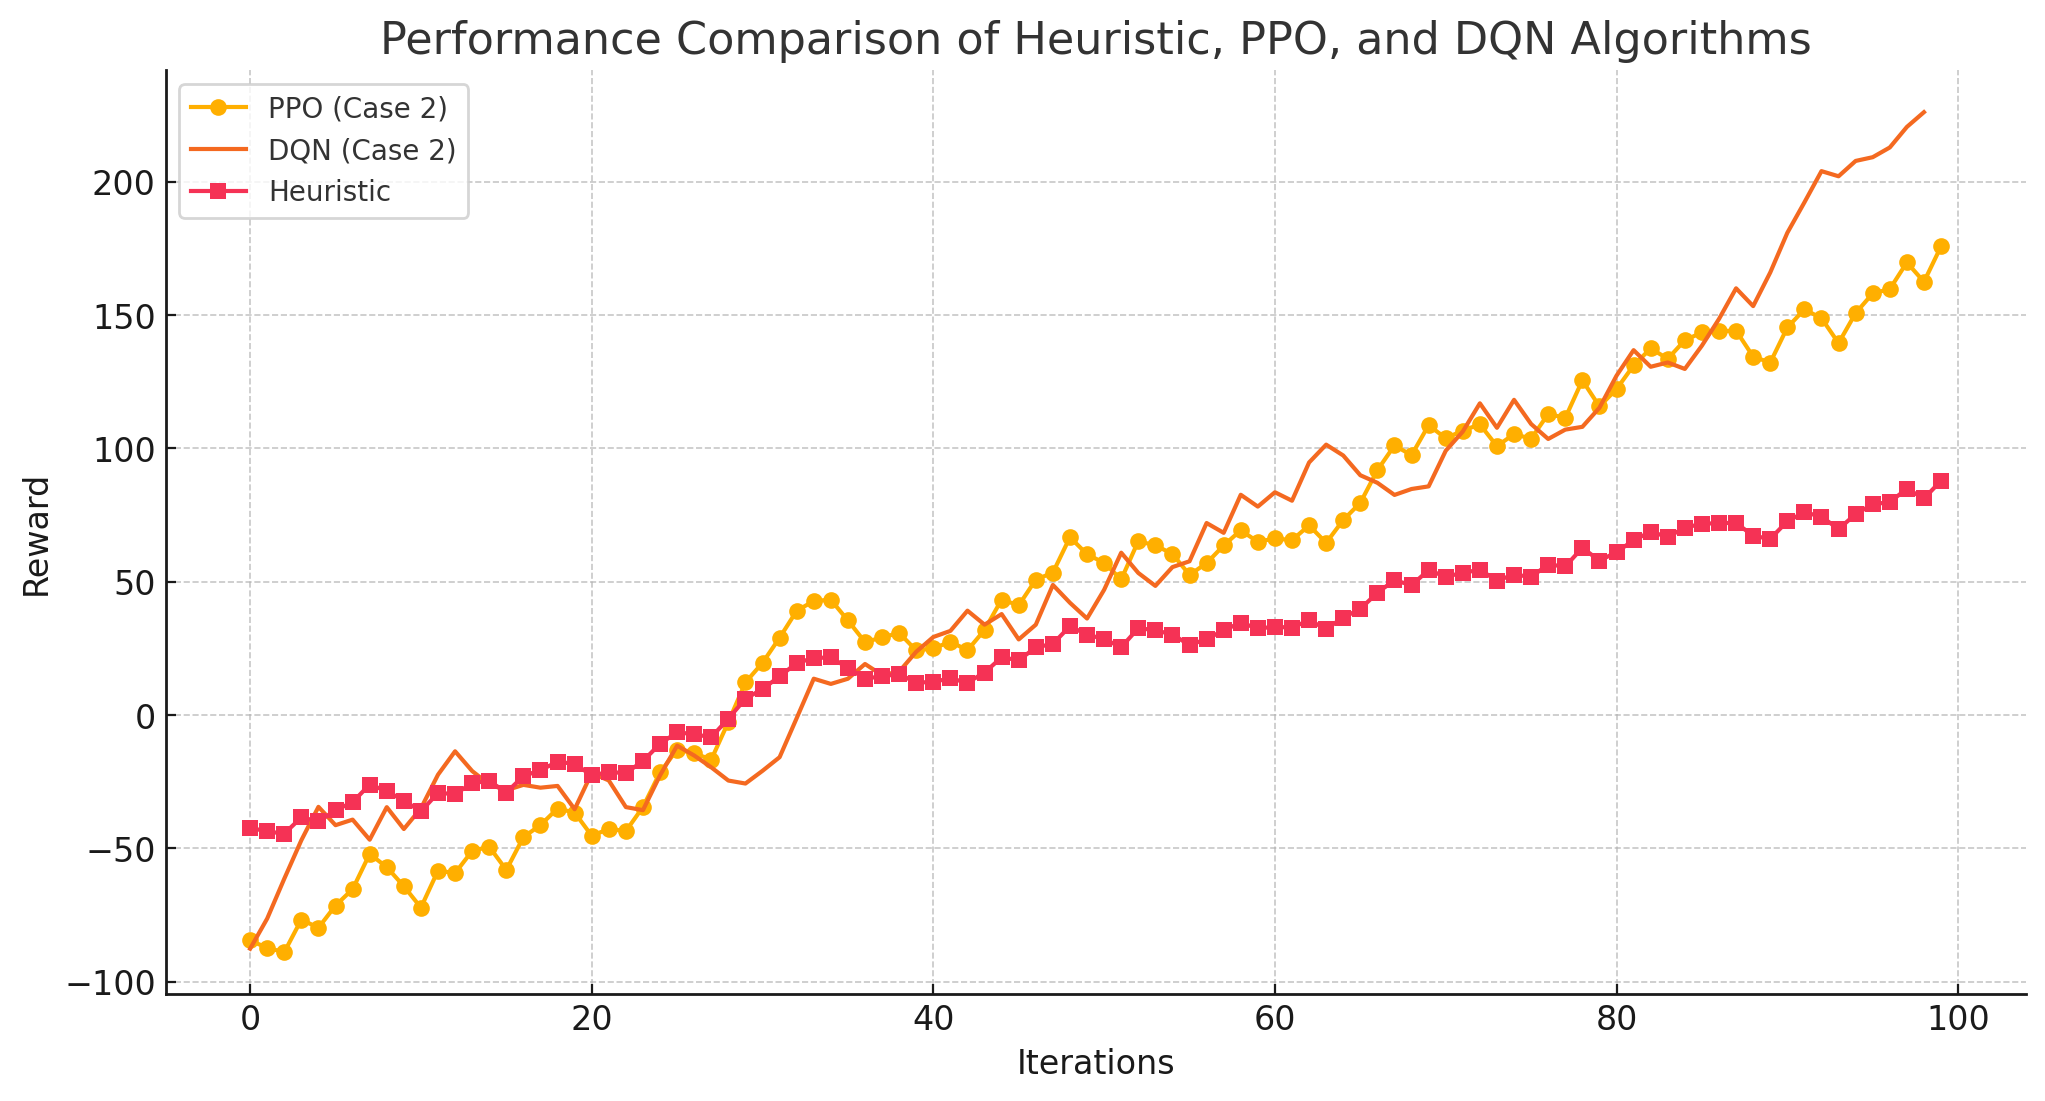
\includegraphics[width=0.8\linewidth]{Fig/heuristic_case1.png}
\caption{Performance comparison of Heuristic, PPO, and DQN algorithms (Case 1).}
\label{fig:heuristic_case1}
\end{figure}
Fig.1 shows the performance comparison of Heuristic, PPO, and DQN algorithms for Case 1. It demonstrates how the rewards evolve over iterations, highlighting the efficiency of RL methods in learning optimal routing strategies.

\begin{figure}[h]
\centering
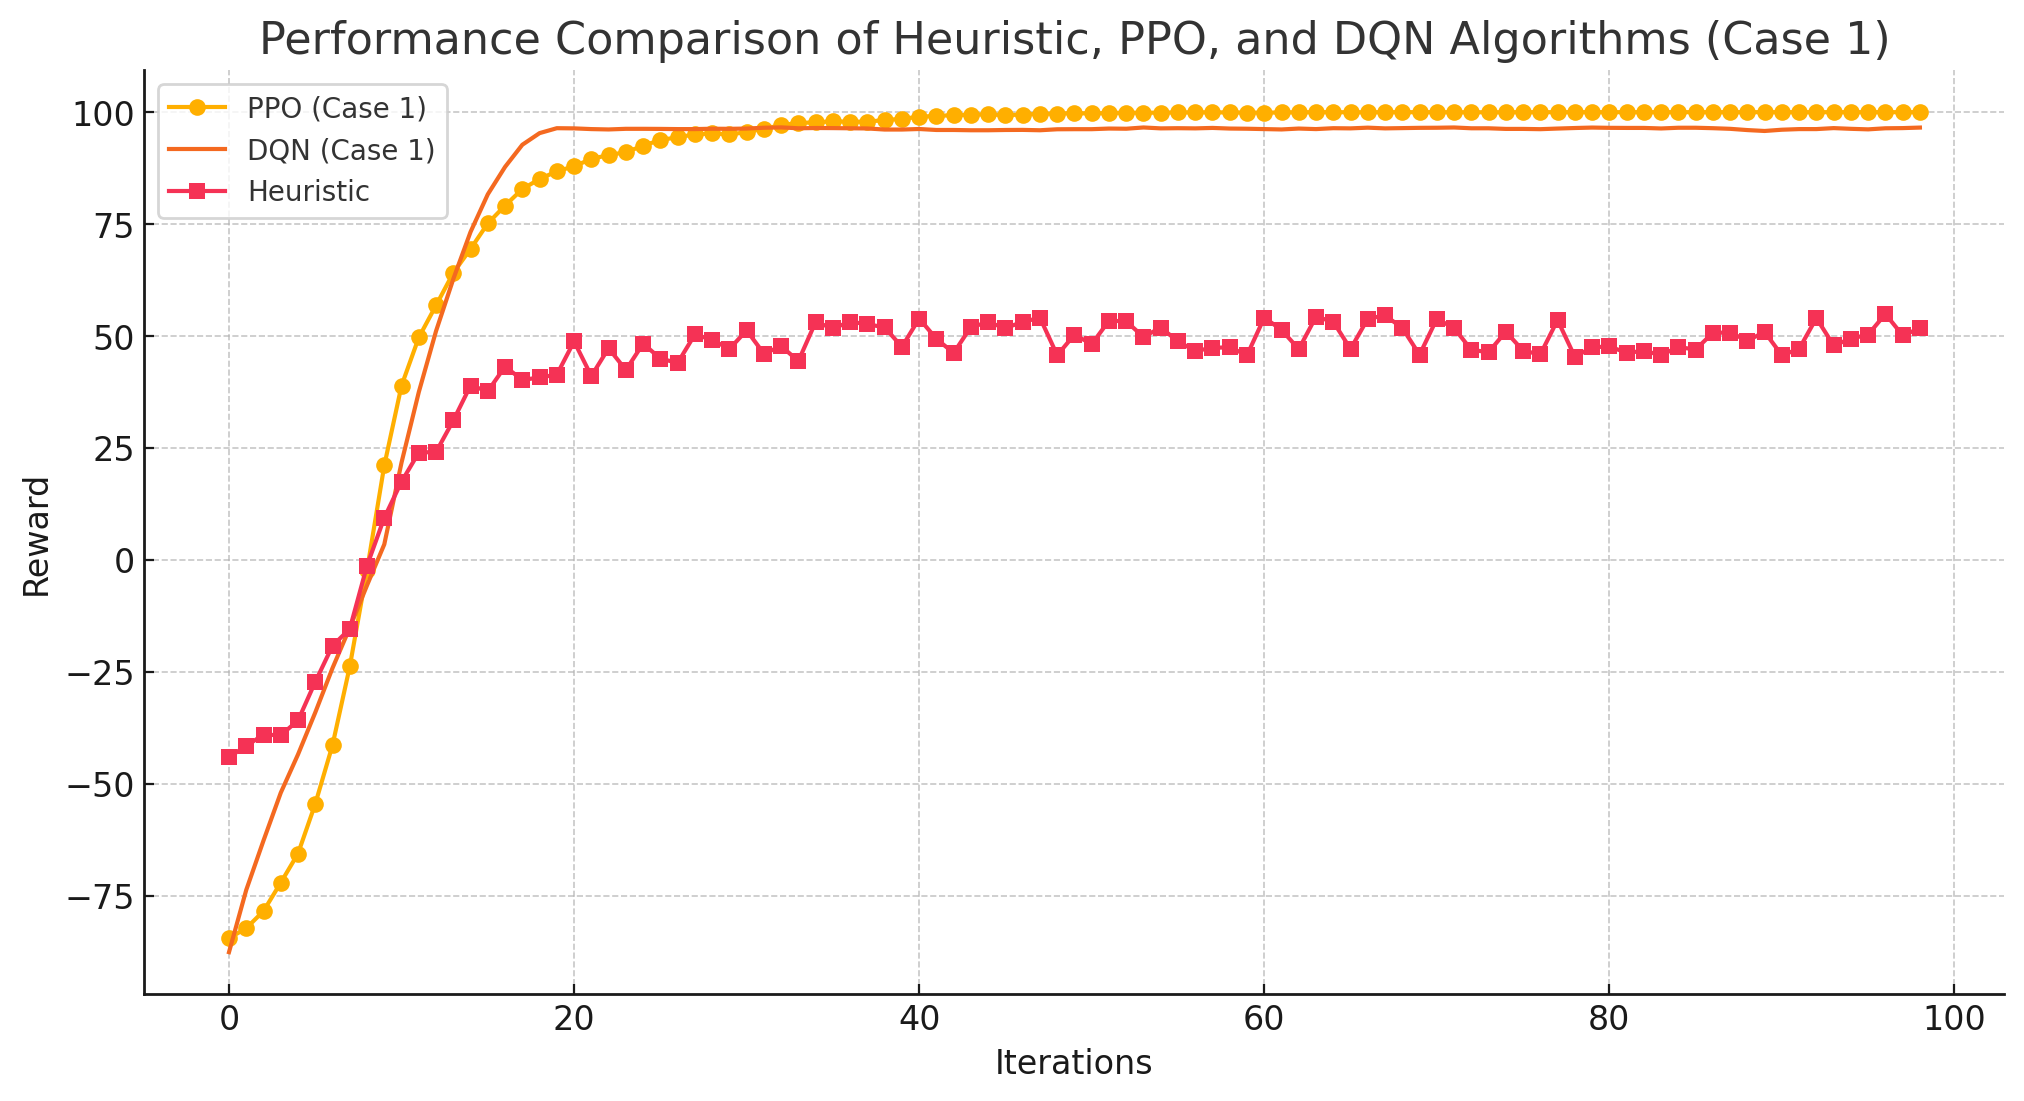
\includegraphics[width=0.8\linewidth]{Fig/heuristic2.png}
\caption{Performance comparison of Heuristic, PPO, and DQN algorithms (Case 2).}
\label{fig:heuristic_case2}
\end{figure}
Fig.2 shows the performance comparison of Heuristic, PPO, and DQN algorithms for Case 2. It highlights the adaptability of RL methods to different traffic patterns, showcasing their robustness in various scenarios.

\begin{figure}[h]
\centering
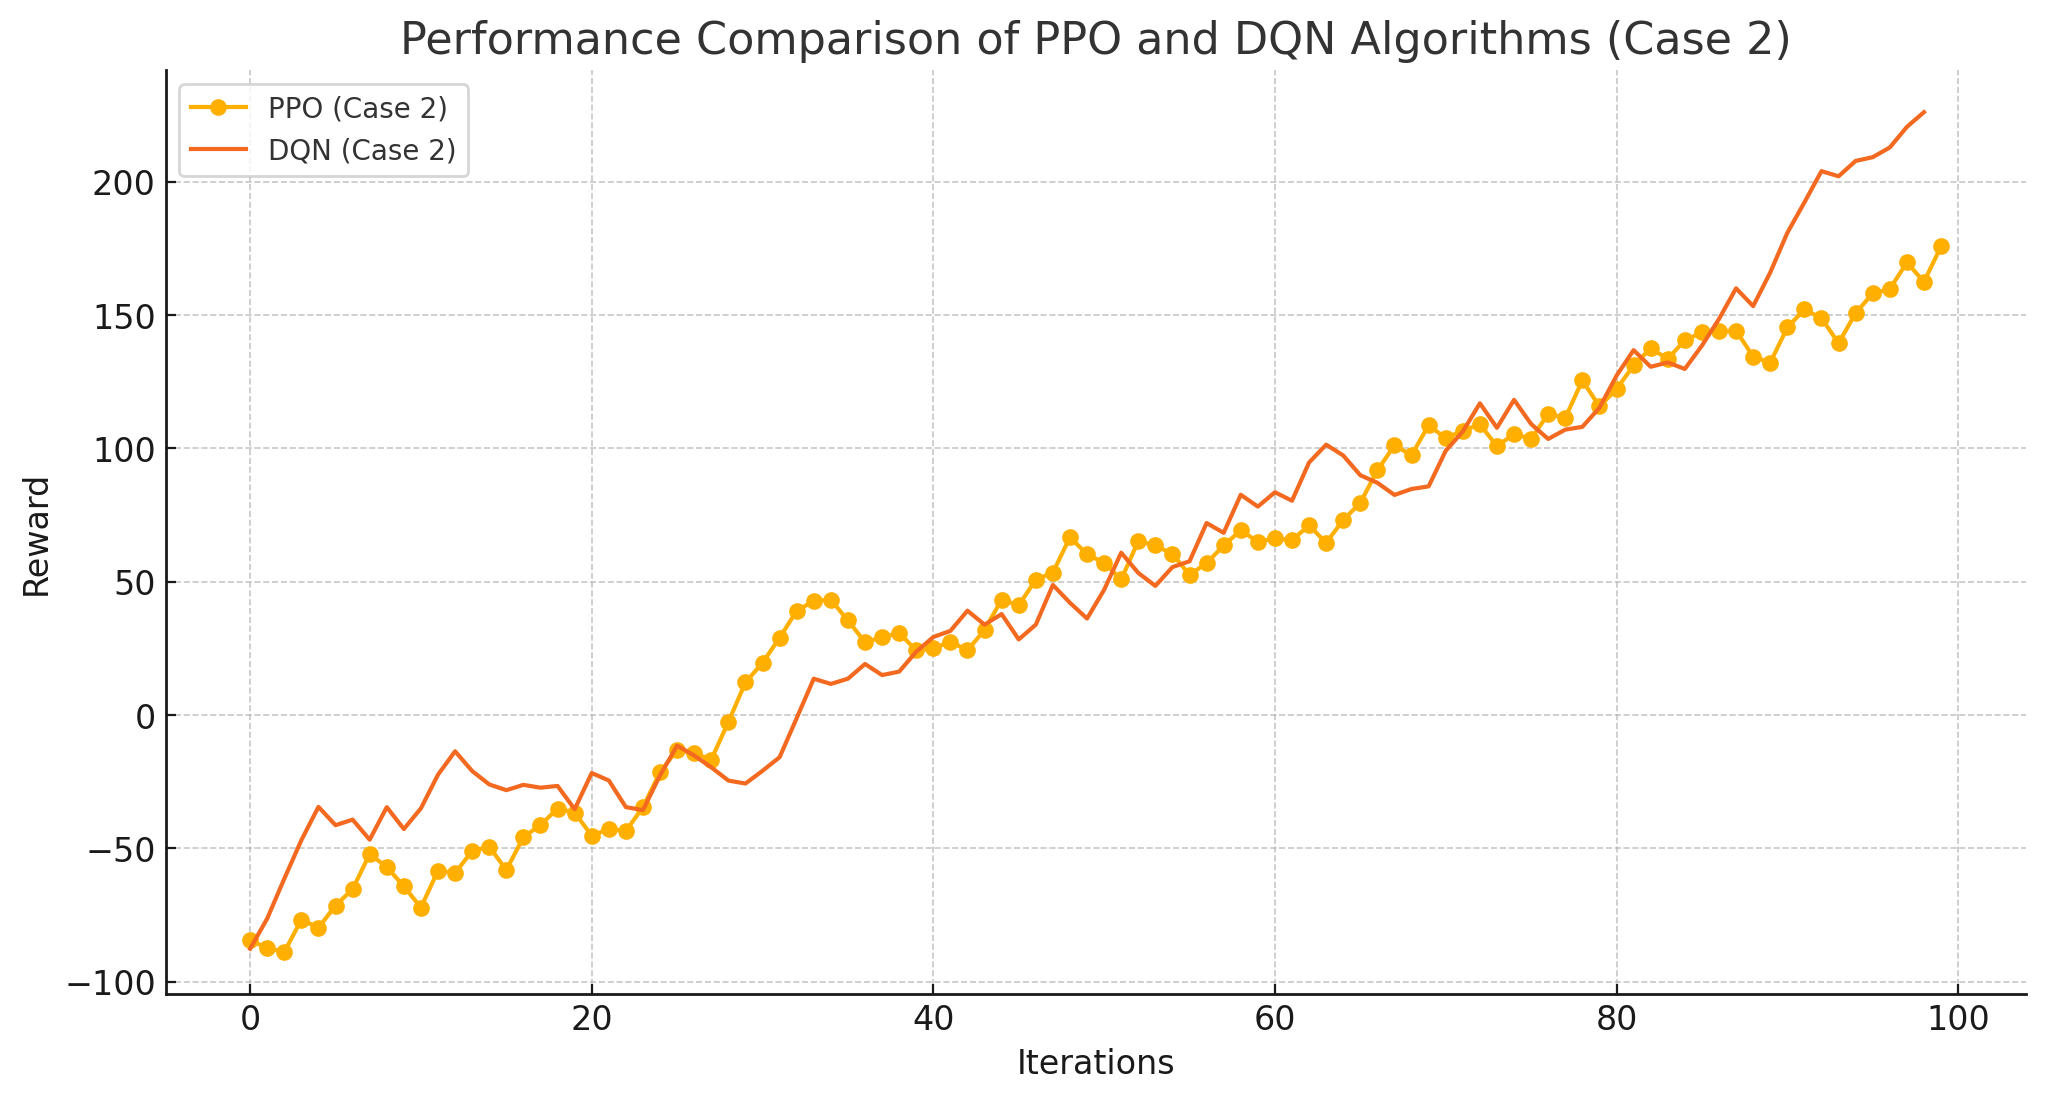
\includegraphics[width=0.8\linewidth]{Fig/PPOvs DQN cas2.png}
\caption{Performance comparison of PPO and DQN algorithms (Case 2).}
\label{fig:ppo_dqn_case2}
\end{figure}
Fig.3 compares the performance of PPO and DQN specifically for Case 2, illustrating their convergence patterns. Both algorithms show significant improvement over time, with DQN exhibiting a slightly higher variance in rewards.

\begin{figure}[h]
\centering
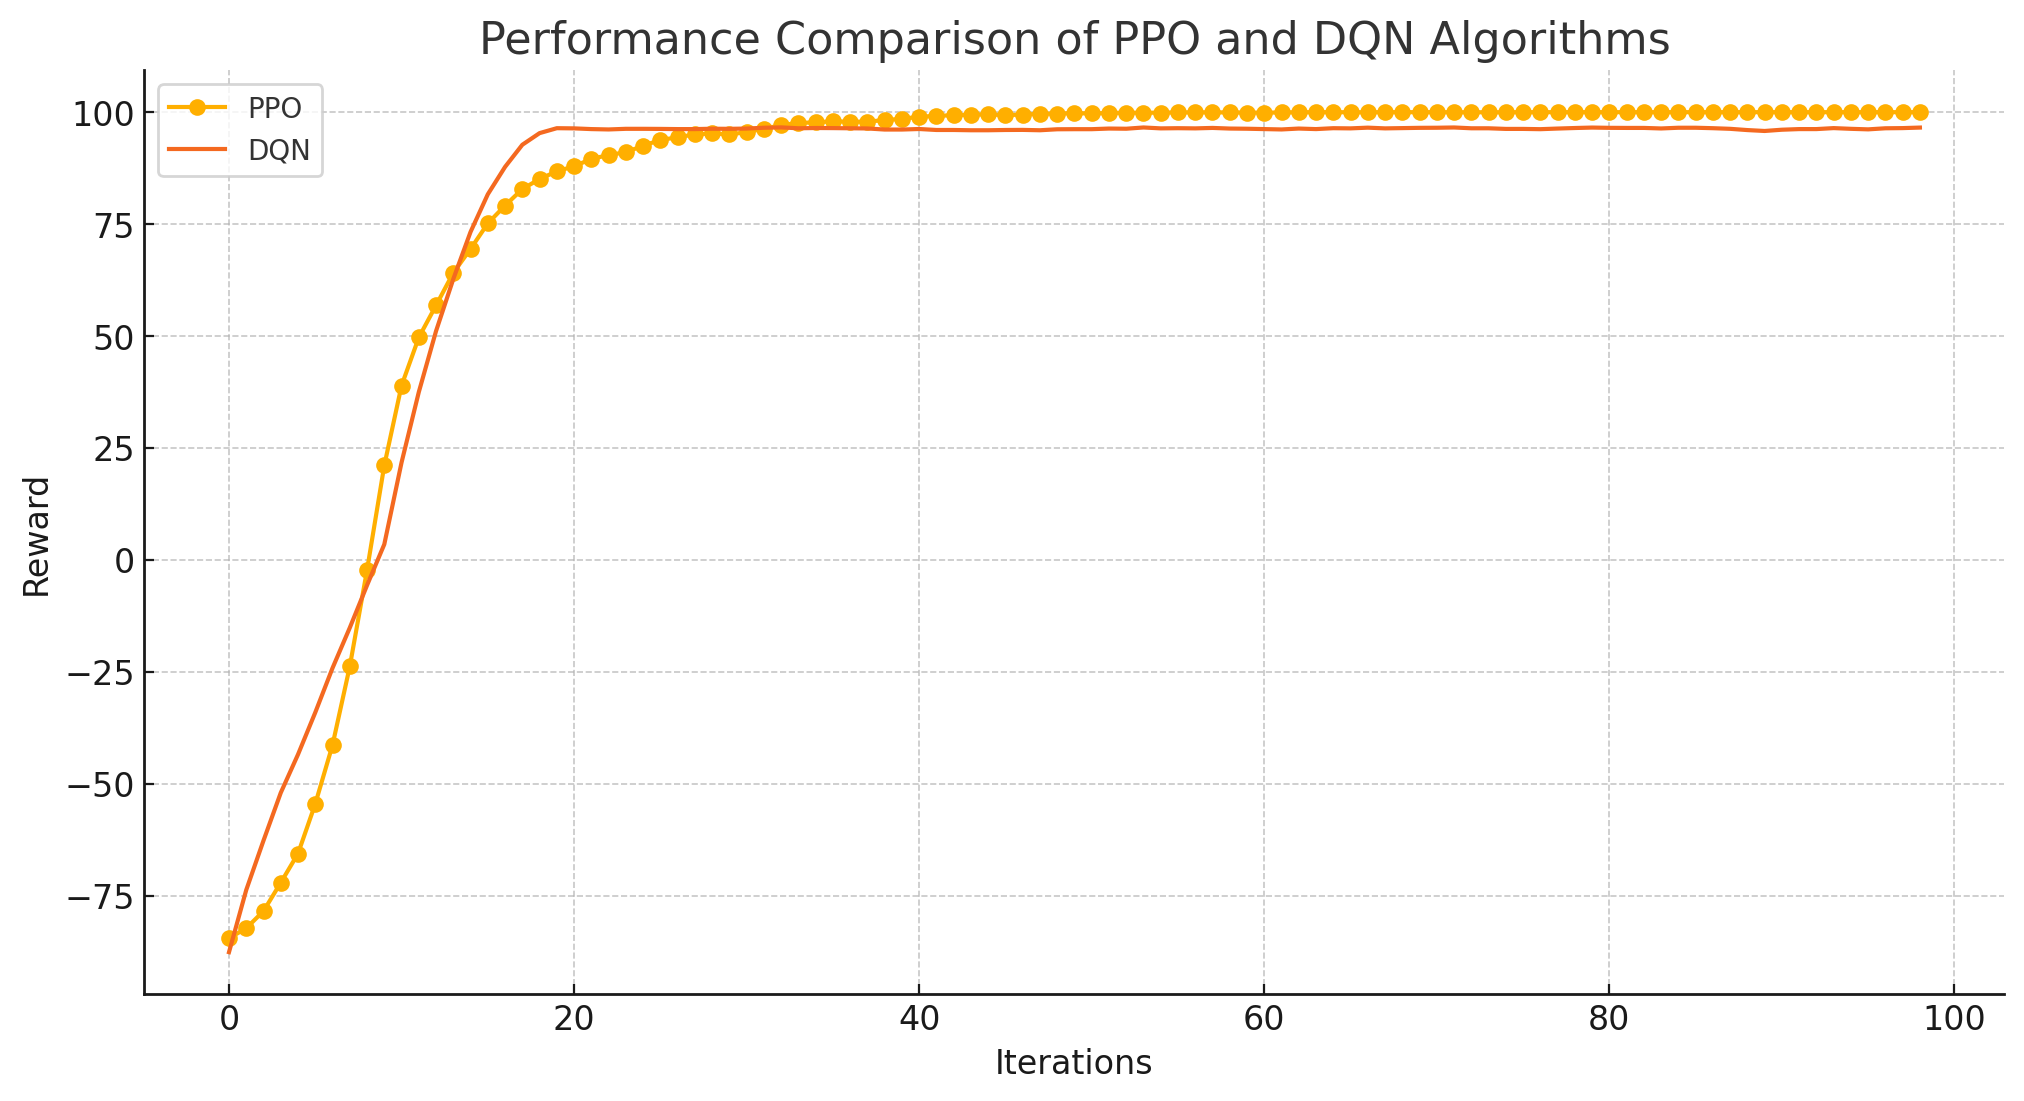
\includegraphics[width=0.8\linewidth]{Fig/PPOvsDQN.png}
\caption{Performance comparison of PPO and DQN algorithms.}
\label{fig:ppo_dqn}
\end{figure}
Fig.4 provides a general comparison of PPO and DQN, showing their overall performance improvement over time. Both algorithms converge to high reward values, indicating their effectiveness in optimizing network utilization.

The results show that both PPO and DQN algorithms outperform the heuristic algorithm. This can be attributed to the following reasons:
\begin{itemize}
    \item \textbf{Adaptability}: RL algorithms continuously learn and adapt to the changing network conditions, which allows them to discover and exploit more efficient routing strategies.
    \item \textbf{Exploration and Exploitation}: PPO and DQN balance exploration of new routing paths and exploitation of known successful paths, leading to better overall performance.
    \item \textbf{Learning from Experience}: RL algorithms improve over time as they learn from the rewards and penalties received for successful and blocked requests, respectively. This learning process is not present in the heuristic algorithm, which follows a static strategy.
\end{itemize}


\section{Conclusion}
The RL-based routing methods (PPO and DQN) demonstrate significant improvements in network utilization compared to the heuristic algorithm. PPO and DQN effectively learn optimal routing strategies that minimize blocking and maximize utilization. The heuristic algorithm, while simpler, provides a useful benchmark for evaluating the RL-based methods. These results highlight the potential of RL in optimizing complex network environments.

\bibliographystyle{ieeetr}
\bibliography{ref}

\begin{itemize}
    \item [1] Sutton, R. S., \& Barto, A. G. (2018). Reinforcement Learning: An Introduction. MIT Press.
    \item [2] Schulman, J., Wolski, F., Dhariwal, P., Radford, A., \& Klimov, O. (2017). Proximal Policy Optimization Algorithms. arXiv preprint arXiv:1707.06347.
    \item [3] Mnih, V., Kavukcuoglu, K., Silver, D., Rusu, A. A., Veness, J., Bellemare, M. G., ... \& Hassabis, D. (2015). Human-level control through deep reinforcement learning. Nature, 518(7540), 529-533.
    \item [4] Li, Y., \& Malik, M. (2017). An overview of machine learning in communications: A tutorial. IEEE Communications Surveys \& Tutorials, 19(2), 855-876.
\end{itemize}

\end{document}
